\documentclass[prd,showpacs,twocolumn]{revtex4-1}
\usepackage{graphicx}% Include figure files
\usepackage{epstopdf}
\usepackage{dcolumn}% Align table columns on decimal point
\usepackage{bm}% bold math
\usepackage{amsmath}
%\nofiles
\begin{document}
\title{Experiments testing Bell's inequality with local real source}
\author{Peifeng Wang}
\email{peifeng\_w@yahoo.com}
\address{Mijiaqiao 34-1-3-5, Xi'an, Shaanxi, P. R. China 710075}
\address{Guanghua Road 1\#, 34-1-3-5, Yanta District, Xi'an, Shaanxi, P. R. China 710075}
\begin{abstract}
Aside from Bell's inequality, QM and local real theory have other specifications that can be observed in experiments. To explore these specifications, we re-examine EPR paradox to show that non-locality arises from the absence of location variable. Our analysis are then applied to several reported experiments. 1) In a known short range Bell experiment with high detection efficiency, portion of the presented data agrees more with local real model than with QM. 2) The so called non maximally entangled state in several experiments are essentially partially entangled photons, with a large local real part helping the violation of Bell's inequality, and the reported event counts deviate from expected entanglement model. 3) In long range EPR experiments for closing locality loophole, interactions with local real apparatus prior to measurements put the entanglement in question.
\end{abstract}
\pacs{03.65.Ud}
\maketitle
%249489

Bell's inequality\cite{Bell,CHSH}/entanglement has been extensively studied\cite{Aspect,Weihs, Rowe, Cavalcanti, Branciard} as it distinguishes quantum mechanics(QM) from local real theories. In a typical setup in testing Bell's inequality as shown in fig. \ref{fig:General}, the source produces entangled particle pairs, which are measured by Alice and Bob. Various experiments have been reported to violate Bell's inequality, in support of QM while ruling out local real theory.

\begin{figure}
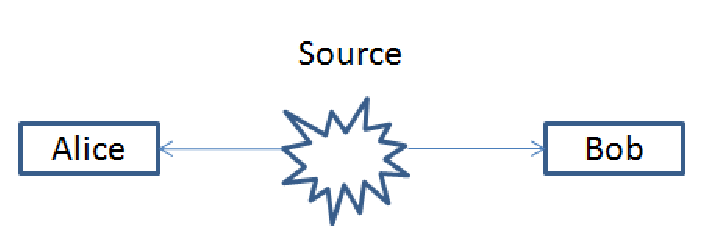
\includegraphics[scale=0.7]{general-png.eps}
\caption{General setup of a Bell experiment}
\label{fig:General}
\end{figure}

But in addition to Bell's inequality, QM and local real theory have other empirical specifications which are expected to be consistent with a valid experiments. To study these various specifications, we first re-examine EPR paradox\cite{EPR} to reveal the origin of non-locality as lack of location variable $\mathbf x$ in wave function, which is thus incapable of modelling interaction with local real apparatus. Several experiments are analyzed, in a short range Bell experiment with high detection efficiency, portion of the presented data agrees more with local real model than with QM. In many other experiments, the so called non-maximally entangled photons are essentially partially entangled, which oddly involves a substantial local real part in the source to help violation of Bell's inequality, and the reported event counts deviate from the expected entanglement model. Then in many long range experiments for closing locality loophole, the interactions with local real device can not be properly modelled by the non-local wave function, thus the measurements in these experiments are only taken on local real photons.

To some extent, EPR paradox can be explained without ``spooky action at a distance". Due to uncertainty principle $\Delta x\Delta p > \frac{\hbar}{2}$, when Alice measures the particle momentum on the left side, $\Delta p_A=0$, $\Delta x_A$ becomes infinitely large, so $x_A$ can take any value. i.e. the particle measured by Alice can be anywhere, in specific, it can just be next to its peer particle on the right side and have an intimate impact on $p_B$ and $x_B$.

The above arguments may seem rhetoric, but it reveals the origin of non locality. The infinitely large $\Delta x$ effectively removes the location variable from an equation. With location variable $\mathbf x$ absent, the equation would be incapable of treating local real interactions happening at a particular location with a definite amount of impact, and thus would be non local.

If an equation lacks a variable that has substantial impact on the physical process to be described, the equation becomes indefinite and incomplete. For example, if an actual physical process varies with respect to location $\mathbf x$, but an equation $\mathcal E$ attempting to describe the physical process lacks location variable $\mathbf x$, then in $\mathcal E$'s expression, the physical process assumes a set of values uniformly over the entire space (rather than a unique value at each $\mathbf x$), or alternatively, $\mathcal E$ represents the physical process as a non-local superposition. Likewise, if time variable is absent, instantaneity also means eternity.

While subsequent studies on the topic focus on particle spin instead of position/momentum pair, QM, in its eigenvalue/eigenstate interpretation, factors out the location variable from wave function, which is thus non local. As to be shown later, the non local wave function is inadequate to describe many reported experiments.

In the following discussion, $\alpha$ is the polarization of the detector at Alice's side of an EPR experiment, $P_A$ is the probability measured at Alice's side. On Bob's side, $\beta$ is the polarization of the detector and $P_B$ is the probability.

With a local real source, a pair of photons with identical polarization are sent to Alice and Bob. The polarization $\theta$ of the photons is defined before it is measured. As Alice and Bob each has a location specification, they are at different locations, thus their detection outcomes can not be directly correlated. Instead, Alice and Bob can each calculate the correlation between the polarization of their own detectors and the photon polarization $\theta$.

When Alice measures the photon with a detector of polarization $\alpha$, the probabilities of detection result are
\begin{eqnarray}
&&P_A(1|\theta,\alpha)=cos^2(\theta-\alpha)\nonumber\\
&&P_A(0|\theta,\alpha)=sin^2(\theta-\alpha)
\label{eqn:PA}
\end{eqnarray}

Similarly on Bob's side, where the photon is measured with a detector in polarization $\beta$
\begin{eqnarray}
&&P_B(1|\theta,\beta)=cos^2(\theta-\beta)\nonumber\\
&&P_B(0|\theta,\beta)=sin^2(\theta-\beta)
\label{eqn:PB}
\end{eqnarray}
the probability of $\theta$ is evenly distributed
\begin{eqnarray}
&&P_A(\theta|\alpha)=\frac{1}{2\pi}
\end{eqnarray}
then the joint conditional probability
\begin{eqnarray}
&&P_A(1,\theta|\alpha)=P_A(1|\theta,\alpha)P_A(\theta|\alpha)=\frac{1}{2\pi}cos^2(\theta-\alpha)
\end{eqnarray}

The local real joint probability of Alice detecting a 1 photon at polarization $\alpha$ and Bob detecting a 1 photon at polarization $\beta$ can be derived with eqn. (\ref{eqn:PB}),
\begin{eqnarray}
P_{local-real}(1,1|\alpha,\beta)&&=\int_0^{2\pi} P_B(1|\theta,\beta)P_A(\theta,1|\alpha)d\theta\nonumber\\
&&=\int_0^{2\pi} \frac{1}{2\pi}cos^2(\theta-\alpha)cos^2(\theta-\beta)d\theta\nonumber\\
&&=\frac{1}{8}+ \frac{1}{4}cos^2(\alpha-\beta)
\label{eqn:PLocalReal}
\end{eqnarray}
similarly,
\begin{eqnarray}
P_{local-real}(0,0|\alpha,\beta)&&=\frac{1}{8}+ \frac{1}{4}cos^2(\alpha-\beta)\nonumber\\
P_{local-real}(0,1|\alpha,\beta)&&=\frac{1}{8}+ \frac{1}{4}sin^2(\alpha-\beta)\nonumber\\
P_{local-real}(1,0|\alpha,\beta)&&=\frac{1}{8}+ \frac{1}{4}sin^2(\alpha-\beta)
\label{eqn:PLocalReal1}
\end{eqnarray}

Unlike the above local real model, entangled photon pair are in a quantum singlet state
\begin{eqnarray}
\left| \Psi\right >=\frac{1}{\sqrt{2}}(\left| 1\right>_A\left| 1\right>_B+\left| 0\right>_A\left| 0\right>_B)
\label{eqn:Singlet}
\end{eqnarray}

In this quantum setup, the photon polarization $\theta$ does not exist, and as photons do not have location specification, their polarization can be directly correlated. The quantum joint probability of Alice detecting a 1 photon at polarization $\alpha$ and Bob detecting a 1 photon at polarization $\beta$ can be derived directly from eqn. (\ref{eqn:Singlet})
\begin{eqnarray}
P_{QM}(1,1|\alpha,\beta)&&=\frac{1}{2}cos^2(\alpha-\beta)
\label{eqn:PQM}
\end{eqnarray}
similarly,
\begin{eqnarray}
P_{QM}(0,0|\alpha,\beta)&&=\frac{1}{2}cos^2(\alpha-\beta)\nonumber\\
P_{QM}(0,1|\alpha,\beta)&&=\frac{1}{2}sin^2(\alpha-\beta)\nonumber\\
P_{QM}(1,0|\alpha,\beta)&&=\frac{1}{2}sin^2(\alpha-\beta)
\label{eqn:PQM1}
\end{eqnarray}

\begin{figure}
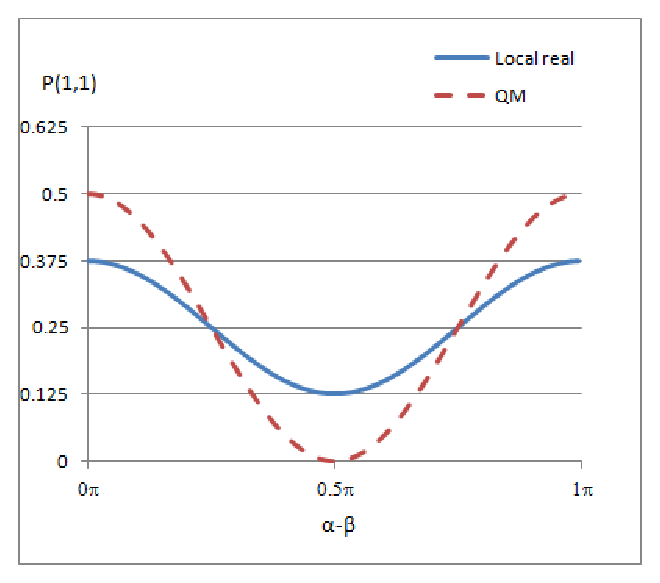
\includegraphics[scale=0.7]{prob-png.eps}
\caption{Joint probability of detecting 1 at both Alice's and Bob's sides}
\label{fig:Probability}
\end{figure}

For comparison, eqn. (\ref{eqn:PLocalReal}) and (\ref{eqn:PQM}) are plotted in fig. \ref{fig:Probability}. As it shows, sinusoidal shaped joint probability is predicted by both QM and local real model. The primary difference is the range of the probability, which enables various inequalities to be constructed. Consequently, it is important to compute the actual probability in any experiment testing Bell's inequality. And it is error prone in interpreting existing experimental data. For example:

1) Subtracting accidental coincidences could shift the sinusoidal curve.

2) Both sinusoidal curves in fig. \ref{fig:Probability} are about probability. In the QM model, $P_{QM}(1,1|\alpha,\beta)$ has a maximal value of 0.5, which is important in violation of Bell's inequality but has never been directly confirmed. Many known experiments reported absolute count of coincidence and plotted them in sinusoidal shaped curve. But without knowledge of the total count, these absolute count can not be accurately mapped to probability and used in Bell test. e.g. if the underlying probability is
\begin{eqnarray}
P_{illustrative}(1,1|\alpha,\beta)=\frac{1}{4}cos^2(\alpha-\beta)
\end{eqnarray}
instead of eqn. (\ref{eqn:PQM}), it can also generate the reported data, but it does not violate Bell's inequality.

To apply above theoretical models in an experiment, the computation of probability needs knowledge of the total number of test runs. Such requirement can only be met in experiments with high detection efficiency. We thus analyze the experiment in \cite{Rowe}, which reports following data:

``a, Data histogram with a negative correlation using $\phi_1 = 3\pi/8$ and $\phi_2 = 3\pi/8$. For these data $N_0 = 2,200$, $N_1 = 15,500$ and $N_2 = 2,300$. b, Data histogram with a positive correlation using $\phi_1 = 3\pi/8$ and $\phi_2 = -\pi/8$. For these data $N_0 = 7,700$, $N_1 = 4,400$ and $N_2 = 7,900$. The zero bright peak extends vertically to 2,551."

The total number of experiment in \cite{Rowe} is 20,000, the above data translate to: a) for negative correlation, $N(0,0) = 2,200$, $N(1,0)+N(0,1) = 15,500$ and $N(1,1) = 2,300$. The probability can be computed:
\begin{eqnarray}
&&P(0,0)=\frac{N(0,0)}{20000}=11\%\nonumber\\
&&P(0,1)+P(1,0)=\frac{N(0,1)+N(1,0)}{20000}=77.5\%\nonumber\\
&&P(1,1)=\frac{N(1,1)}{20000}=11.5\%
\label{eqn:PMassive-}
\end{eqnarray}
b) for positive correlation, $N(0,0) = 7,700$, $N(1,0)+N(0,1) = 4,400$ and $N(1,1) = 7,900$. The probability
\begin{eqnarray}
&&P(0,0)=\frac{N(0,0)}{20000}=38.5\%\nonumber\\
&&P(0,1) + P(1,0)=\frac{N(0,1)+N(1,0)}{20000}=22\%\nonumber\\
&&P(1,1)=\frac{N(1,1)}{20000}=39.5\%
\label{eqn:PMassive+}
\end{eqnarray}

Table \ref{tab:comparison}  compares the above experimental data with predictions from QM and local real model. These data agrees more with local real model than with QM.
\begin{table}
\caption{\label{tab:comparison}Comparison of experimental data from \cite{Rowe} and prediction of QM and local real model}
%\begin{ruledtabular}
\begin{center}
For negative correlation $|\alpha-\beta|=\pi/2$
\begin{tabular}{cccc}
\hline
&Experimental data&QM&local real\\
\hline
P(0,0) & 11\% & 0\% & 12.5\% \\
\hline
P(0,1)+P(1,0) & 77.5\% & 100\% & 75\% \\
\hline
P(1,1) & 11.5\% & 0\% & 12.5\% \\
\hline\\\\
\end{tabular}\\
For positive correlation $|\alpha-\beta|=0$
\begin{tabular}{cccc}
\hline
&Experimental data&QM&local real\\
\hline
P(0,0) & 38.5\% & 50\% & 37.5\% \\
\hline
P(0,1)+P(1,0) & 22\% & 0\% & 25\% \\
\hline
P(1,1) & 39.5\% & 50\% & 37.5\% \\
\hline
\end{tabular}
\end{center}
%\end{ruledtabular}
\end{table}

Although \cite{Rowe} claims violation of Bell's inequality, the presented data gives visibility $V<0.6$, substantially less than the minimal threshold 0.707 required for violation of Bell's inequality, which appears quite intriguing.

Several other experiments attempt to close the fair sampling loophole by using an inequality without requiring fair sampling. However, fair sampling is indispensable in all statistical experiments, because theoretically, all inequalities must deal with some probabilities (e.g. $p_{++}$), whereas experimentally, all tests can only collect raw count of events (e.g. $N_{++},N_{total}$). Normally the probabilities in an inequality are estimated as a ratio of the raw counts collected in an experiment (e.g. $p_{++}=N_{++}/N_{total}$), which is only valid when sampling is fair. Thus fair sampling is always necessary regardless of the inequality being used, unless one is not doing a statistical experiment. It is odd that \cite{Giustina, Shalm} do not require fair sampling.

\cite{Giustina, Shalm} also use non maximally entangled state
\begin{eqnarray}
\left| \Psi\right >&&=\frac{1}{\sqrt{1+r^2}}(\left| 1\right>_A\left| 1\right>_B+r\left| 0\right>_A\left| 0\right>_B)\nonumber\\
&&=\frac{\left| 1\right>_A\left| 1\right>_B+\left| 0\right>_A\left| 0\right>_B}{\sqrt{1+r^2}}+\frac{(r-1)\left| 0\right>_A\left| 0\right>_B}{\sqrt{1+r^2}}\nonumber\\
&&=\left| \Psi\right >_{entangle}+\left| \Psi\right >_{local}
\label{eqn:partialSinglet}
\end{eqnarray}

Eqn. (\ref{eqn:partialSinglet}) actually represents partially entangled photons, which contains a full entanglement part $\left| \Psi\right >_{entangle}$ and a local real part $\left| \Psi\right >_{local}$, each of which contribute to the joint probabilities of the detection outcomes. Here, we use the entanglement part as a rough approximation for the joint probability of partial entanglement wave function
\begin{eqnarray}
P_{partial}(1,1|\alpha,\beta)&&\approx\frac{1}{1+r^2}P_{QM}=\frac{cos^2(\alpha-\beta)}{1+r^2}
\label{eqn:PPartial}
\end{eqnarray}
It is odd that the local real part in the wave function can help violate the selected inequality.

Incidentally, data reported in \cite{Giustina, Shalm} deviate from the joint probability expected from the above partial entanglement model. For example, figure 3 in \cite{Giustina} shows $p_{++}(a_2b_2)<10^{-4}$ with $r=-2.9, \alpha=a_2=62.4^\circ,\beta= b_2=25.5^\circ$, but the joint probability estimated by (\ref{eqn:PPartial}) is about 0.068. From the table S-II in the supplemental material of \cite{Shalm}, the estimated joint probability $p_{++}(ab)=6378/(6378+3289+3147+44336240) = 0.000144$ with $r=3.47, \alpha=a=4.2^\circ, \beta=b=-4.2^\circ$, but the joint probability projected by (\ref{eqn:PPartial}) is about 0.075.

\begin{figure}
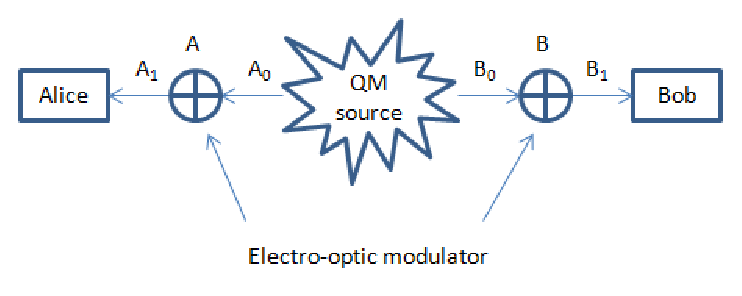
\includegraphics[scale=0.7]{redraw-png.eps}
\caption{Simplified diagram of \cite{Weihs}}
\label{fig:Redraw}
\end{figure}

While the raw data deviates from expected model, many experiments also involve interactions with local real apparatus before Alice and Bob take measurements. To illustrate, a simplified setup of \cite{Weihs} is shown in fig. \ref{fig:Redraw}. In \cite{Weihs}, ``Each of the observers switched the direction of local polarization analysis with a transverse electro-optic modulator." That is, a transverse electro-optic modulator is placed on the path of each arm of the experiment, denoted A and B in fig. \ref{fig:Redraw}. $A_0$ and $B_0$ are reference points before photons from the source pass the modulator, $A_1$ and $B_1$ are reference points after photons from the source pass the modulator,

The scheme in fig. \ref{fig:Redraw} is widely used in closing the locality loophole. Such setup has to be finely aligned so that photons pass through the modulator and the measurement polarizer, otherwise, the modulator does not have any impact on photons that don't pass it and the measurement polarizer can not pick up photons that don't pass it. This implies that the modulator and the measurement polarizer each are local real, i.e. the polarization of the photon is changed only at the location of the modulator by a real amount as a function of an external controlling random signal, and measurement happens precisely at the location of the measurement polarizers.

Two local real apparatus (a modulator and a measurement polarizer) are distinct even if they are enclosed in one measurement station. Thus there exists point $A_1$ and $B_1$ between the two distinct apparatus at each end of the experiment, i.e. on Alice's side, there exists point $A_1$ after the modulator and before the measurement polarizer. A few questions then arise:

1)When the photon of an entangled pair on the left passes modulator A and gets its polarization modulated, does its peer photon on the right get changed instantly? Can one photon of an entangled pair be modulated independently? Does entanglement play any role at the modulator?

2)After passing the modulators, can the photon pair remain entangled at $A_1$ and $B_1$? Are Alice's and Bob's polarizers measuring entangled photons? What is the wave function on which Alice and Bob take measurement?

The difficulties are, 1)if entanglement plays no role at the modulator, how can it subsequently have any impact when the photons pass the measurement polarizers? 2) if entanglement plays some role at the modulator, then the photon pair are already disentangled when arriving at Alice's and Bob's measurement polarizers. What did Alice and Bob measure?

These questions expose the incompleteness of the wave function (\ref{eqn:Singlet}). We attempt 2 possible ways of treating electro-optic modulator with QM wave function, in both cases, Alice and Bob are measuring local real photons.

First, wave function (\ref{eqn:Singlet}) remains non-local, i.e. lacks location variable $\mathbf x$, thus it attempts to represent the physical process uniformly in the entire space, regardless of before/after the photon passing the modulator. In this case, the wave function collapses due to interaction with the electro-optic modulator, because if the wave function did not collapse, it (lacking location variable $\mathbf x$) would not be able to describe the change of polarization due to the interaction with electro-optic modulator at location A and B.

With wave function collapsing due to interaction with the modulators at location A and B, Alice and Bob are only left to take measurement on disentangled photons.

Second, we annotate the wave function with location, so the wave function can reflect the change of polarization introduced by the local real modulator A and B. In such annotations, the wave function becomes local to some extent.

If the wave function at $A_0$ and $B_0$ is in entanglement,
\begin{eqnarray}
\left| \Psi\right >_{A_0, B_0}=\frac{1}{\sqrt{2}}(\left| 1\right>_A\left| 1\right>_B+\left| 0\right>_A\left| 0\right>_B)
\label{eqn:AnnotatedSinglet}
\end{eqnarray}
the wave function at $A_1$ and $B_1$ must be different than (\ref{eqn:AnnotatedSinglet}) to reflect the change of polarization due to electro-optic modulator. As the electro-optic modulator can be arbitrarily configured by the controlling random signal, the wave function at $A_1$ and $B_1$ will contain all possible joint states, thus becomes
\begin{eqnarray}
\left| \Psi\right >_{A_1, B_1}=\left| 1\right>_A\left| 1\right>_B+\left| 0\right>_A\left| 0\right>_B + \left| 1\right>_A\left| 0\right>_B+\left| 1\right>_A\left| 0\right>_B\nonumber\\
\label{eqn:Disturbed}
\end{eqnarray}
the wave function at $A_1, B_1$ is in disentanglement, Alice and Bob are only measuring disentangled photons.

The above arguments arises when the non-local wave function needs to model the change of polarization due to the local real electro-optic modulator in the experiment. The same analysis applies when the non-local wave function has to treat the interaction with any local real physical model in an actual experiment. In another example, magnetic field has a local real model in that the field has a real value at every location. When a particle interacts with magnetic field, its spin becomes real. Earth is surrounded in its magnetic field, so in all experiments performed on the surface of the Earth, the spin of charged particles are local real. Thus within the Earth's magnetic field, experiments based on the spin of charged particles are only measuring local real quantities.

In general, a local real apparatus exerts a definite amount of impact at a specified location, which can not be modelled by non-local QM wave function. For experiments involving local real apparatus, the wave function on which Alice and Bob are taking measurements is merely in disentanglement, thus local real.

While Bell's inequality presents a statistic to test the local realism hypothesis, the physical essence of entanglement is specified with certainty that, for 2 entities once in interaction and later separated, impact on one entity will instantaneously change the other entity. 

There has been extensive interest in studying Bell's inequality, but the real fundamental question is about the physical essence of entanglement. If one could directly observe the spooky action at a distance, it would be a conclusive support of entanglement, which would leave test of Bell's inequality superfluous. If on the other hand, an experiment has many aspects manifesting local realism (the opposite to entanglement), simple violation of Bell's inequality may not be effective.

In experiments that use partially entangled photons with a substantial local real part to help violating Bell's inequality, that report event counts deviating from joint probability expected in the entanglement model, that rely on interaction with local real apparatus to close locality loophole, the reported violation of Bell's inequality can not be a convincing evidence of entanglement.

\acknowledgments

\begin{thebibliography}{0}

\bibitem{Bell} J. S. Bell, Physics (Long Island City, N. Y.) 1, 195 (1965).
\bibitem{CHSH} J. F. Clauser, M. A. Horne, A. Shimony, and R. A. Holt, \emph{Phys. Rev. Lett.} 23, 880 (1969).
\bibitem{Aspect} A. Aspect, J. Dalibard, and G. Roger, Phys. Rev. Lett. 49, 1804 (1982).
\bibitem{Weihs} G. Weihs, T. Jennewein, C. Simon, H. Weinfurter, and A. Zeilinger, Phys. Rev. Lett. 81, 5039 (1998).
\bibitem{Rowe} M. A. Rowe, D. Kielpinski, V. Meyer, C. A. Sackett, W. M. Itano, C. Monroe, and D. J. Wineland, Nature (London) 409, 791 (2001).
\bibitem{Cavalcanti} E. G. Cavalcanti, C. J. Foster, M. D. Reid, and P. D. Drummond, Phys. Rev. Lett. 99, 210405 (2007)
\bibitem{Branciard} C. Branciard, A. Ling, N. Gisin, C. Kurtsiefer, A. Lamas-Linares, and V. Scarani, Phys. Rev. Lett. 99, 210407 (2007)
\bibitem{EPR} A. Einstein, B. Podolosky, and N. Rosen, Phys. Rev. 47, 777 (1935).
\bibitem{Giustina} M. Giustina et al., Phys. Rev. Lett. 115, 250401 (2015)
\bibitem{Shalm} L. K. Shalm et al., Phys. Rev. Lett. 115, 250402 (2015)
\end{thebibliography}

\end{document}

